\documentclass[journal,12pt,twocolumn]{IEEEtran}
\usepackage{setspace}
\usepackage{gensymb}
\usepackage{caption}
%\usepackage{multirow}
%\usepackage{multicolumn}
%\usepackage{subcaption}
%\doublespacing
\singlespacing
\usepackage{csvsimple}
\usepackage{amsmath}
\usepackage{multicol}
%\usepackage{enumerate}
\usepackage{amssymb}
%\usepackage{graphicx}
\usepackage{newfloat}
%\usepackage{syntax}
\usepackage{listings}
\usepackage{iithtlc}
\usepackage{color}
\usepackage{tikz}
\usetikzlibrary{shapes,arrows}



%\usepackage{graphicx}
%\usepackage{amssymb}
%\usepackage{relsize}
%\usepackage[cmex10]{amsmath}
%\usepackage{mathtools}
%\usepackage{amsthm}
%\interdisplaylinepenalty=2500
%\savesymbol{iint}
%\usepackage{txfonts}
%\restoresymbol{TXF}{iint}
%\usepackage{wasysym}
\usepackage{amsthm}
\usepackage{mathrsfs}
\usepackage{txfonts}
\usepackage{stfloats}
\usepackage{cite}
\usepackage{cases}
\usepackage{mathtools}
\usepackage{caption}
\usepackage{enumerate}	
\usepackage{enumitem}
\usepackage{amsmath}
%\usepackage{xtab}
\usepackage{longtable}
\usepackage{multirow}
%\usepackage{algorithm}
%\usepackage{algpseudocode}
\usepackage{enumitem}
\usepackage{mathtools}
\usepackage{hyperref}
%\usepackage[framemethod=tikz]{mdframed}
\usepackage{listings}
    %\usepackage[latin1]{inputenc}                                 %%
    \usepackage{color}                                            %%
    \usepackage{array}                                            %%
    \usepackage{longtable}                                        %%
    \usepackage{calc}                                             %%
    \usepackage{multirow}                                         %%
    \usepackage{hhline}                                           %%
    \usepackage{ifthen}                                           %%
  %optionally (for landscape tables embedded in another document): %%
    \usepackage{lscape}     


\usepackage{url}
\def\UrlBreaks{\do\/\do-}


%\usepackage{stmaryrd}


%\usepackage{wasysym}
%\newcounter{MYtempeqncnt}
\DeclareMathOperator*{\Res}{Res}
%\renewcommand{\baselinestretch}{2}
\renewcommand\thesection{\arabic{section}}
\renewcommand\thesubsection{\thesection.\arabic{subsection}}
\renewcommand\thesubsubsection{\thesubsection.\arabic{subsubsection}}

\renewcommand\thesectiondis{\arabic{section}}
\renewcommand\thesubsectiondis{\thesectiondis.\arabic{subsection}}
\renewcommand\thesubsubsectiondis{\thesubsectiondis.\arabic{subsubsection}}

% correct bad hyphenation here
\hyphenation{op-tical net-works semi-conduc-tor}

%\lstset{
%language=C,
%frame=single, 
%breaklines=true
%}

%\lstset{
	%%basicstyle=\small\ttfamily\bfseries,
	%%numberstyle=\small\ttfamily,
	%language=Octave,
	%backgroundcolor=\color{white},
	%%frame=single,
	%%keywordstyle=\bfseries,
	%%breaklines=true,
	%%showstringspaces=false,
	%%xleftmargin=-10mm,
	%%aboveskip=-1mm,
	%%belowskip=0mm
%}

%\surroundwithmdframed[width=\columnwidth]{lstlisting}
\def\inputGnumericTable{}                                 %%
\lstset{
%language=C,
frame=single, 
breaklines=true,
columns=fullflexible
}
 

\begin{document}
%
\tikzstyle{block} = [rectangle, draw,
    text width=3em, text centered, minimum height=3em]
\tikzstyle{sum} = [draw, circle, node distance=3cm]
\tikzstyle{input} = [coordinate]
\tikzstyle{output} = [coordinate]
\tikzstyle{pinstyle} = [pin edge={to-,thin,black}]

\theoremstyle{definition}
\newtheorem{theorem}{Theorem}[section]
\newtheorem{problem}{Problem}
\newtheorem{proposition}{Proposition}[section]
\newtheorem{lemma}{Lemma}[section]
\newtheorem{corollary}[theorem]{Corollary}
\newtheorem{example}{Example}[section]
\newtheorem{definition}{Definition}[section]
%\newtheorem{algorithm}{Algorithm}[section]
%\newtheorem{cor}{Corollary}
\newcommand{\BEQA}{\begin{eqnarray}}
\newcommand{\EEQA}{\end{eqnarray}}
\newcommand{\define}{\stackrel{\triangle}{=}}

\bibliographystyle{IEEEtran}
%\bibliographystyle{ieeetr}

\providecommand{\nCr}[2]{\,^{#1}C_{#2}} % nCr
\providecommand{\nPr}[2]{\,^{#1}P_{#2}} % nPr
\providecommand{\mbf}{\mathbf}
\providecommand{\pr}[1]{\ensuremath{\Pr\left(#1\right)}}
\providecommand{\qfunc}[1]{\ensuremath{Q\left(#1\right)}}
\providecommand{\sbrak}[1]{\ensuremath{{}\left[#1\right]}}
\providecommand{\lsbrak}[1]{\ensuremath{{}\left[#1\right.}}
\providecommand{\rsbrak}[1]{\ensuremath{{}\left.#1\right]}}
\providecommand{\brak}[1]{\ensuremath{\left(#1\right)}}
\providecommand{\lbrak}[1]{\ensuremath{\left(#1\right.}}
\providecommand{\rbrak}[1]{\ensuremath{\left.#1\right)}}
\providecommand{\cbrak}[1]{\ensuremath{\left\{#1\right\}}}
\providecommand{\lcbrak}[1]{\ensuremath{\left\{#1\right.}}
\providecommand{\rcbrak}[1]{\ensuremath{\left.#1\right\}}}
\theoremstyle{remark}
\newtheorem{rem}{Remark}
\newcommand{\sgn}{\mathop{\mathrm{sgn}}}
\providecommand{\abs}[1]{\left\vert#1\right\vert}
\providecommand{\res}[1]{\Res\displaylimits_{#1}} 
\providecommand{\norm}[1]{\left\Vert#1\right\Vert}
\providecommand{\mtx}[1]{\mathbf{#1}}
\providecommand{\mean}[1]{E\left[ #1 \right]}
\providecommand{\fourier}{\overset{\mathcal{F}}{ \rightleftharpoons}}
%\providecommand{\hilbert}{\overset{\mathcal{H}}{ \rightleftharpoons}}
\providecommand{\system}{\overset{\mathcal{H}}{ \longleftrightarrow}}
	%\newcommand{\solution}[2]{\textbf{Solution:}{#1}}
\newcommand{\solution}{\noindent \textbf{Solution: }}
\newcommand{\myvec}[1]{\ensuremath{\begin{pmatrix}#1\end{pmatrix}}}
\providecommand{\dec}[2]{\ensuremath{\overset{#1}{\underset{#2}{\gtrless}}}}
\DeclarePairedDelimiter{\ceil}{\lceil}{\rceil}
%\numberwithin{equation}{section}
%\numberwithin{problem}{subsection}
%\numberwithin{definition}{subsection}
\makeatletter
\@addtoreset{figure}{section}
\makeatother

\let\StandardTheFigure\thefigure
%\renewcommand{\thefigure}{\theproblem.\arabic{figure}}
\renewcommand{\thefigure}{\thesection}


%\numberwithin{figure}{subsection}

%\numberwithin{equation}{subsection}
%\numberwithin{equation}{section}
%\numberwithin{equation}{problem}
%\numberwithin{problem}{subsection}
\numberwithin{problem}{section}
%%\numberwithin{definition}{subsection}
%\makeatletter
%\@addtoreset{figure}{problem}
%\makeatother
\makeatletter
\@addtoreset{table}{section}
\makeatother

\let\StandardTheFigure\thefigure
\let\StandardTheTable\thetable
\let\vec\mathbf
\numberwithin{equation}{section}

\vspace{3cm}


\title{%Convex Optimization in Python
	\logo{
	Random Numbers
	}
}
%\title{
%	\logo{Matrix Analysis through Octave}{\begin{center}\includegraphics[scale=.24]{tlc}\end{center}}{}{HAMDSP}
%}


% paper title
% can use linebreaks \\ within to get better formatting as desired
%\title{Matrix Analysis through Octave}
%
%
% author names and IEEE memberships
% note positions of commas and nonbreaking spaces ( ~ ) LaTeX will not break
% a structure at a ~ so this keeps an author's name from being broken across
% two lines.
% use \thanks{} to gain access to the first footnote area
% a separate \thanks must be used for each paragraph as LaTeX2e's \thanks
% was not built to handle multiple paragraphs
%

\author{Rishit D$^{*}$% <-this % stops a space
}% <-this % stops a space
%\thanks{J. Doe and J. Doe are with Anonymous University.}% <-this % stops a space
%\thanks{Manuscript received April 19, 2005; revised January 11, 2007.}}
}
% note the % following the last \IEEEmembership and also \thanks - 
% these prevent an unwanted space from occurring between the last author name
% and the end of the author line. i.e., if you had this:
% 
% \author{....lastname \thanks{...} \thanks{...} }
%                     ^------------^------------^----Do not want these spaces!
%
% a space would be appended to the last name and could cause every name on that
% line to be shifted left slightly. This is one of those "LaTeX things". For
% instance, "\textbf{A} \textbf{B}" will typeset as "A B" not "AB". To get
% "AB" then you have to do: "\textbf{A}\textbf{B}"
% \thanks is no different in this regard, so shield the last } of each \thanks
% that ends a line with a % and do not let a space in before the next \thanks.
% Spaces after \IEEEmembership other than the last one are OK (and needed) as
% you are supposed to have spaces between the names. For what it is worth,
% this is a minor point as most people would not even notice if the said evil
% space somehow managed to creep in.



% The paper headers
%\markboth{Journal of \LaTeX\ Class Files,~Vol.~6, No.~1, January~2007}%
%{Shell \MakeLowercase{\textit{et al.}}: Bare Demo of IEEEtran.cls for Journals}
% The only time the second header will appear is for the odd numbered pages
% after the title page when using the twoside option.
% 
% *** Note that you probably will NOT want to include the author's ***
% *** name in the headers of peer review papers.                   ***
% You can use \ifCLASSOPTIONpeerreview for conditional compilation here if
% you desire.




% If you want to put a publisher's ID mark on the page you can do it like
% this:
%\IEEEpubid{0000--0000/00\$00.00~\copyright~2007 IEEE}
% Remember, if you use this you must call \IEEEpubidadjcol in the second
% column for its text to clear the IEEEpubid mark.



% make the title area
\maketitle

\tableofcontents

\bigskip

\renewcommand{\thefigure}{\theenumi}
\renewcommand{\thetable}{\theenumi}

\begin{abstract}
Solutions to Random Numbers
\end{abstract}
%%

\section{Uniform Random Numbers}
Let $U$ be a uniform random variable between 0 and 1.
\begin{enumerate}[label=\thesection.\arabic*
,ref=\thesection.\theenumi]
\item Generate $10^6$ samples of $U$ using a C program and save into a file called uni.dat .
\\
\solution Download the following files. 
\begin{lstlisting}
wget https://github.com/gadepall/probability/raw/master/manual/codes/exrand.c
wget https://github.com/gadepall/probability/raw/master/manual/codes/coeffs.h
\end{lstlisting}

Now execute the following code.
\begin{lstlisting}
gcc exrand.c -lm
./a.out
\end{lstlisting}

%
\item
Load the uni.dat file into python and plot the empirical CDF of $U$ using the samples in uni.dat. The CDF is defined as
\begin{align}
F_{U}(x) = \pr{U \le x}
\end{align}
\\
\solution  The following code plots Fig. \ref{fig:uni_cdf}
\begin{lstlisting}
wget https://github.com/gadepall/probability/raw/master/manual/codes/cdf_plot.py
python3 cdf_plot.py
\end{lstlisting}
\begin{figure}[!ht]
\centering
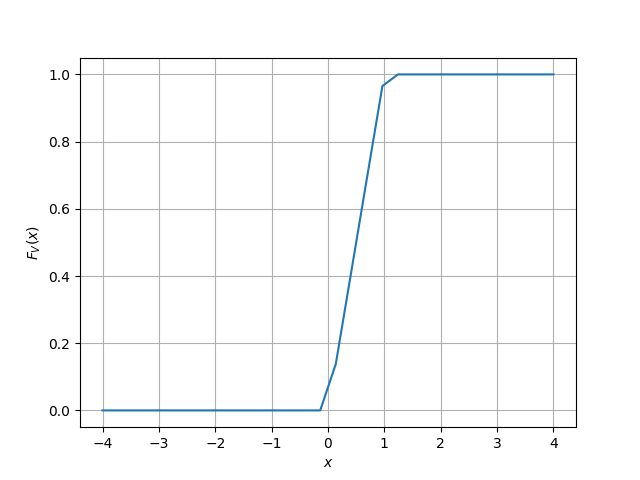
\includegraphics[width=\columnwidth]{../figs/uni_cdf.png}
\caption{The CDF of $U$}
\label{fig:uni_cdf}
\end{figure}

%
\item
Find a theoretical expression for $F_{U}(x)$.
\\
\solution Given $U$ is a uniformly distributed random variable over the interval $(0, 1)$, we have the density function $p_U(x)$:

	\begin{align}
		p_U(x) = 
		\begin{cases}
			1, & x \in (0, 1) \\
			0, & otherwise
		\end{cases}
		\label{eq:PDF_U}
	\end{align}
	
	We know

	\begin{align}
		F_U(x) = \int_{-\infty}^{x} p_U(x) \,dx
		\label{eq:Relation}
	\end{align}
	
	Given $U$ is a uniformly distributed random variable over the interval $(0, 1)$, we have the following expression for $F_U(x)$:
	
	\begin{align}
		F_U(x) = 
		\begin{cases}
			0, & x \in (-\infty, 0) \\
      			x, & x \in (0, 1) \\
      			1, & x \in (1, \infty)
    		\end{cases}
	\end{align}

\item
The mean of $U$ is defined as
%
\begin{equation}
E\sbrak{U} = \frac{1}{N}\sum_{i=1}^{N}U_i
\end{equation}
%
and its variance as
%
\begin{equation}
\text{var}\sbrak{U} = E\sbrak{U- E\sbrak{U}}^2 
\end{equation}

Write a C program to  find the mean and variance of $U$.
\\
\solution
\\
Execute the following commands on linux terminal:
\begin{lstlisting}
gcc mean_var_uni.c -lm
./a.out
\end{lstlisting}

\item Verify your result theoretically given that
\end{enumerate}
%
\begin{align}
E\sbrak{U^k} = \int_{-\infty}^{\infty}x^kdF_{U}(x)
\end{align}
\\
\solution
This can be alternatively wriiten as
	\begin{align}
		E[U^k] = \int^{\infty}_{-\infty} x^k p_U(x) \,dx
		\label{eq: Expected}
	\end{align}

We know that mean $\mu$ is given by $E(U)$. Hence
	\begin{align}
		\mu = \int_{-\infty}^{\infty} x p_U(x) \,dx
		\label{eq:Relation_1}
	\end{align}

	\begin{align}
		\mu &= \int_{0}^{1} x \,dx \\
		&= \frac{x^2}{2} \Bigg|^{1}_{0} \\
		&= \fbox{$\frac{1}{2}$} 
		\label{eq: Mean}
	\end{align}
	
We know
	\begin{align}
		var(U) = E((U - E(U))^2)
	\end{align}

	This can also be represented as
	\begin{align}
		var(U) &= E(U^2 - 2E(U)U + (E(U))^2) \\
		&= E(U^2) - 2(E(U))^2 + (E(U))^2 \\
		&= E(U^2) - (E(U))^2
		\label{eq: Relation_2}
	\end{align}

We can evaluate $E(U^2)$ using \eqref{eq: Expected} as:
	\begin{align}
		E(U^2) &= \int_{-\infty}^{\infty} x^2 p_U(x) \,dx \\
		&= \int_{0}^{1} x^2 \,dx \\
		&= \frac{x^3}{3} \Bigg|^{1}_{0} \\
		&= \frac{1}{3}
	\end{align}

Using \eqref{eq: Mean} and \eqref{eq: Relation_2} we have
	\begin{align}
		var(U) = \frac{1}{3} - \frac{1}{4} = \fbox{$\frac{1}{12}$}
	\end{align}

Using this, we obtain mean as $0.5007$ and variance as $0.083301$. Hence the statistically obtained values are in close agreement with the theoretical values of $\mu = 0.5$ and $\sigma^2 = \frac{1}{12}$.


\section{Central Limit Theorem}
%
\begin{enumerate}[label=\thesection.\arabic*
,ref=\thesection.\theenumi]

%
\item
Generate $10^6$ samples of the random variable
%
\begin{equation}
X = \sum_{i=1}^{12}U_i -6
\end{equation}
%
using a C program, where $U_i, i = 1,2,\dots, 12$ are  a set of independent uniform random variables between 0 and 1
and save in a file called gau.dat.
\\
\solution
To generate samples for the Gaussian distribution, run the following code
\begin{lstlisting}
gcc exrand.c -lm
./a.out
\end{lstlisting}

%
\item
Load gau.dat in python and plot the empirical CDF of $X$ using the samples in gau.dat. What properties does a CDF have?
\\
\solution The CDF of $X$ is plotted in Fig. \ref{fig:gauss_cdf}
\begin{figure}
\centering
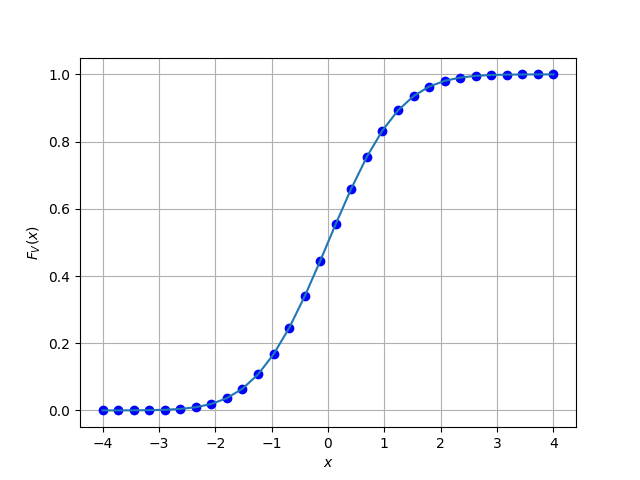
\includegraphics[width=\columnwidth]{../figs/gau_cdf.png}
\caption{The CDF of $X$}
\label{fig:gauss_cdf}
\end{figure}


\item
Load gau.dat in python and plot the empirical PDF of $X$ using the samples in gau.dat. The PDF of $X$ is defined as
\begin{align}
p_{X}(x) = \frac{d}{dx}F_{X}(x)
\end{align}
What properties does the PDF have?
\\
\solution The PDF of $X$ is plotted in Fig. \ref{fig:gauss_pdf} using the code below
\begin{lstlisting}
wget https://github.com/gadepall/probability/raw/master/manual/codes/pdf_plot.py
python3 pdf_plot.py
\end{lstlisting}

\begin{figure}
\centering
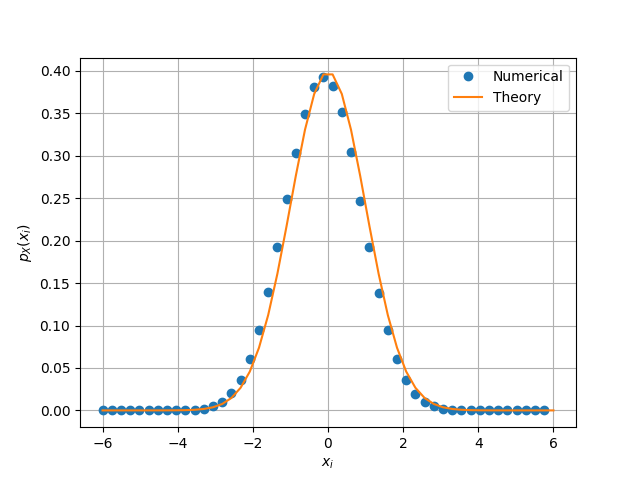
\includegraphics[width=\columnwidth]{../figs/gauss_pdf.png}
\caption{The PDF of $X$}
\label{fig:gauss_pdf}
\end{figure}

\item Find the mean and variance of $X$ by writing a C program.
\\
\solution
\\
The mean and variance is given by the following code:
\begin{lstlisting}
gcc mean_var_gau.c -lm
./a.out
\end{lstlisting}

\item Given that 
\begin{align}
p_{X}(x) = \frac{1}{\sqrt{2\pi}}\exp\brak{-\frac{x^2}{2}}, -\infty < x < \infty,
	\label{eq:PDF_2}
\end{align}
repeat the above exercise theoretically.
\\
\solution Given
	\begin{align}
		F_X(x) = \int_{-\infty}^{x} p_X(x) \,dx
		\label{eq:Relation_3}
	\end{align}

	We have, using 
	\eqref{eq:Relation_3} and 
	\eqref{eq:PDF_2}
	\begin{align}
		F_X(x) = \int_{-\infty}^{x} \frac{1}{\sqrt{2\pi}}\exp{\left(-\frac{x^2}{2}\right)} \,dx
		\label{eq:CDFInt}
	\end{align}
	
	The Q-Function is defined as follows:
	\begin{align}
		Q(x) &= \Pr(X > x) \\
		&= 1 - \Pr(X \leq x)
		\label{eq:QFunc}
	\end{align}

	Hence, using \eqref{eq:QFunc}, we can write
	\begin{align}
		F_X(x) &= \Pr(X \leq x) \\
		&= 1 - Q(x)
		\label{eq:FinalCDF}
	\end{align}

	Mean for random variable $X$ is given by:
	
	\begin{align}
		\mu_x &= E(X) \\
		&= \int^{\infty}_{-\infty} x p_X(x) \,dx \\
		&= \int^{\infty}_{-\infty} \frac{x}{\sqrt{2\pi}}\exp{\left(-\frac{x^2}{2}\right)} \,dx \\
		&= \fbox{0}
	\end{align}

	Note that the integral
	\begin{align}
		\int^a_{-a} f(x) \,dx
	\end{align}
	becomes 0, when $f(x)$ is odd.
	
	Variance for random variable $X$ is given by:

	\begin{align}
		var(X) = E(X^2) - (E(X))^2
		\label{eq: MeanVar}
	\end{align}

	We evaluate $E(X^2)$ as follows:

	\begin{align}
		E(X^2) &= \int^{\infty}_{-\infty} x^2 p_X(x) \,dx \\
	\end{align}

	Using integration by parts, we have:
	\begin{align}
		E(X^2) &= -x\sqrt{\frac{2}{\pi}} e^{\left(-\frac{x^2}{2}\right)}\Bigg|_{-\infty}^{\infty} +  \int^{\infty}_{-\infty} \sqrt{\frac{2}{\pi}} e^{\left(-\frac{x^2}{2}\right)} \,dx \\
		&= 1
		\label{eq: MeanSec}
	\end{align}

	Hence using \eqref{eq: MeanVar} and \eqref{eq: MeanSec}, we have

	\begin{align}
		var(X) &= E(X^2) - (E(X))^2 \\
		&= 1 - 0^2 \\
		&= \fbox{1}
	\end{align}
Using this, we obtain the statistical mean and variance to be 0.000326 and 1.000906 respectively which is in close agreement with the theoretical values.

	%
\end{enumerate}
\section{From Uniform to Other}
\begin{enumerate}[label=\thesection.\arabic*
,ref=\thesection.\theenumi]
%
\item
Generate samples of 
%
\begin{equation}
V = -2\ln\brak{1-U}
\end{equation}
%
and plot its CDF.
\\
\solution
The following can be used to generate samples for random variable $V$:
\begin{lstlisting}
gcc new_v.c -lm
.\a.out
\end{lstlisting}

The following code can be used to generate CDF for $V$:
\begin{lstlisting}
python3 log_cdf.py
\end{lstlisting}
The figure generated is shown as \eqref{fig:log_cdf}

\begin{figure}
\centering
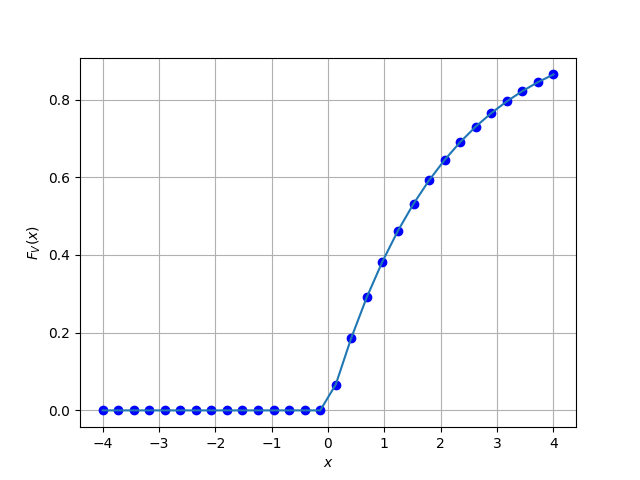
\includegraphics[width=\columnwidth]{../figs/log_cdf.png}
\caption{The PDF of $V$}
\label{fig:log_cdf}
\end{figure}
  
\item Find a theoretical expression for $F_V(x)$.
\\
\solution
We have been given that random variable $V$ is a function of the random variable $U$ as follows:
	
	\begin{align}
		V = -2\ln{(1 - U)}
		\label{eq:FuncRV}
	\end{align}

	Note that the obtained distribution function (CDF) for random variable $U$ is:

	\begin{align}
		F_U(x) = 
		\begin{cases}
			0, & x \in (-\infty, 0) \\
			x, & x \in (0, 1) \\
			1, & x \in (1, \infty)
		\end{cases}
		\label{eq:CDF_U}
	\end{align}

We know for any random variable $X$

	\begin{align}
		F_X(x) = \Pr(X \leq x)
		\label{eq:CDF_Def}
	\end{align}

	Hence, we can write using \eqref{eq:FuncRV} and \eqref{eq:CDF_Def}

	\begin{align}
		F_V(x) &= \Pr(V \leq x) \\
		&= \Pr(-2\ln{(1 - U)} \leq x)\\
		&= \Pr(\ln{(1 - U)} \geq -\frac{x}{2}) \\
		&= \Pr(1 - U \geq \exp{\left(-\frac{x}{2}\right)}) \\
		&= \Pr(U \leq 1 - \exp{\left(-\frac{x}{2}\right)}) \\
		&= F_U(1 - \exp{\left(-\frac{x}{2}\right)}) 
		\label{eq:CDF_Rel}
	\end{align}

Note that the function $f(x) = 1 - \exp{\left(-\frac{x}{2}\right)}$ follows:
	\begin{align}
		f(x) \in
		\begin{cases}
			{0}, & x \in (-\infty, 0) \\
			(0, 1) & x \in (0, \infty)
		\end{cases}
	\end{align}

	Hence we can write
	\begin{align}
		F_V(x) = 
		\begin{cases}
			0, & x \in (-\infty, 0) \\
			1 - \exp{\left(-\frac{x}{2}\right)}, & x \in (0, \infty)
    		\end{cases}
	\end{align}

%
\end{enumerate}

\section{Triangular Distribution}
\begin{enumerate}[label=\thesection.\arabic*
,ref=\thesection.\theenumi]
%

\item
	Generate 
	\begin{align}
		T = U_1 + U_2
		\label{eq:TriRV}
	\end{align}
	\\
	\solution
	\\
	Execute the following code to generate samples of random variable $T$ in \verb|tri.dat|:
	\begin{lstlisting}
gcc exrand.c -lm
./a.out
	\end{lstlisting}

\item
	Find the CDF of T.
	\\
	\solution
	\\
	Execute the following code to generate CDF of T.
	\begin{lstlisting}
python3 tri_cdf.py
	\end{lstlisting}

	The CDF is plotted as shown in \eqref{fig:TriCDF_1}
	\begin{figure}
	\centering
	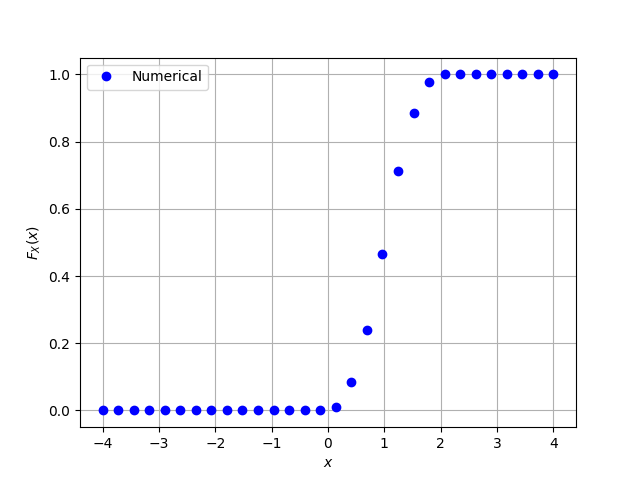
\includegraphics[width=\columnwidth]{../figs/tri_cdf.png}
	\caption{The CDF of $T$}
	\label{fig:TriCDF_1}
	\end{figure}

\item
	Find the PDF of T.
	\\
	\solution
	\\
	Execute the following code to generate PDF of T.
	\begin{lstlisting}
python3 tri_pdf.py
	\end{lstlisting}

	The PDF is plotted as shown in \eqref{fig:TriPDF_1}
	\begin{figure}
	\centering
	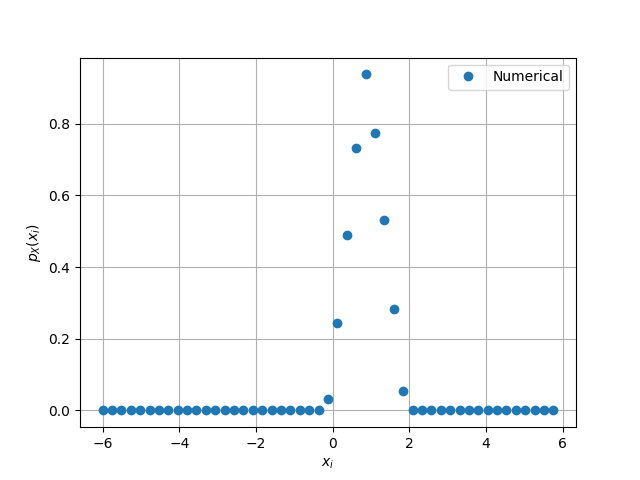
\includegraphics[width=\columnwidth]{../figs/tri_pdf.png}
	\caption{The PDF of $T$}
	\label{fig:TriPDF_1}
	\end{figure}

\item
	Find the theoretical expressions for the PDF and CDF of T.
	\\
	\solution
	\\
	Given a random variable $Z$ as:
	\begin{align}
		Z = X + Y
	\end{align}
	where $X$ and $Y$ are random variables, we can define

	\begin{align}
		p_Z(t) &= p_X(x) * p_Y(y) \\
		&= \int_{-\infty}^{\infty} p_X(\tau) p_Y(t - \tau) \,d\tau
		\label{eq:ConvZ}
	\end{align}

	Given $X = U$, $Y = U$ and $T = X + Y$, we have from \eqref{eq:ConvZ}
	\begin{align}
		p_T(t) &= \int_{-\infty}^{\infty} p_U(\tau) p_U(t - \tau) \,d\tau \\
		&= \int_{0}^{1} p_U(t - \tau) \,d\tau \\
		&= \int_{t-1}^{t} p_U(u) \,du
		\label{eq:T_PDF_Int}
	\end{align}

	From \eqref{eq:PDF_U}, we can deduce that the above integral will be non-zero only when $(t-1, t) \cap (0, 1) \neq \emptyset$. Hence \eqref{eq:T_PDF_1} will be zero when $t < 0$ and $t > 2$.
	
	Consider the integral when $t \in (0, 1)$:
	\begin{align}
		p_T(t) &= \int_{t-1}^{t} p_U(u) \,du \\
		&= \int_{0}^{t} p_U(u) \,du \\
		&= \int_{0}^{t} 1 \,du \\
		&= \fbox{t}
		\label{eq:T_Case1}
	\end{align}

	Consider the integral when $t \in (1, 2)$:
	\begin{align}
		p_T(t) &= \int_{t-1}^{t} p_U(u) \,du \\
		&= \int_{t-1}^{1} p_U(u) \,du \\
		&= \fbox{2-t}
		\label{eq:T_Case2}
	\end{align}

	Hence, we can state $p_T(t)$ as follows from \eqref{eq:T_Case1} and \eqref{eq:T_Case2}:
	\begin{align}
		p_T(t) =
		\begin{cases}
			0, & t \in (-\infty, 0) \\
			t, & t \in (0, 1) \\
			2 - t, & t \in (1, 2) \\
			0, & t \in (0, \infty)
		\end{cases}
		\label{eq:T_PDF}
	\end{align}

	The CDF is related with the PDF as follows:
	\begin{align}
		F_T(t) = \int_{-\infty}^{t} p_T(t) \,dt
		\label{eq:Relation}
	\end{align}

	Using \eqref{eq:Relation}, we have:
	\begin{align}
		F_T(t) =
		\begin{cases}
			0, & t \in (-\infty, 0) \\
			\frac{t^2}{2}, & t \in (0, 1) \\
			\frac{1 - (t-2)^2}{2}, & t \in (1, 2) \\
			1, &t \in (0, \infty)
		\end{cases}
		\label{eq:T_CDF}
	\end{align}

\item
	Verify your result for the PDF through a plot.
	\\
	\solution
	\\
	Execute the following code to generate theoretical and statistical PDF of T.
	\begin{lstlisting}
python3 tri_pdf.py
	\end{lstlisting}
	\begin{figure}
	\centering
	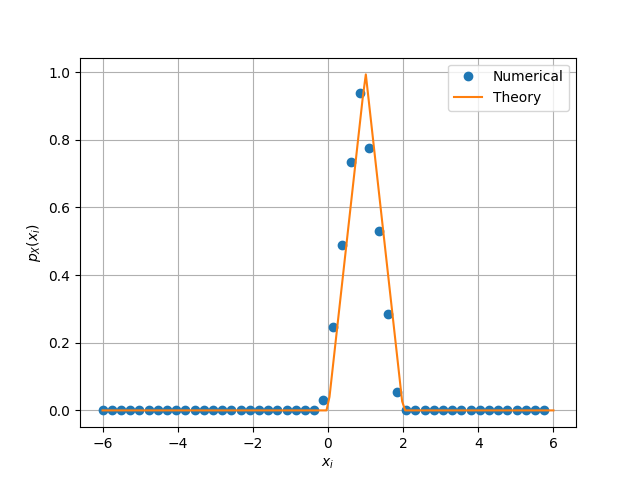
\includegraphics[width=\columnwidth]{../figs/tri_pdf_comp.png}
	\caption{The PDF of $T$}
	\label{fig:TriPDF_2}
	\end{figure}
	
	The plot is shown in figure \eqref{fig:TriPDF_2}.

\item
	Verify your result for the CDF through a plot.
	\\
	\solution
	\\
	Execute the following code to generate theoretical and statistical CDF of T.
	\begin{lstlisting}
python3 tri_cdf.py
	\end{lstlisting}
	\begin{figure}
	\centering
	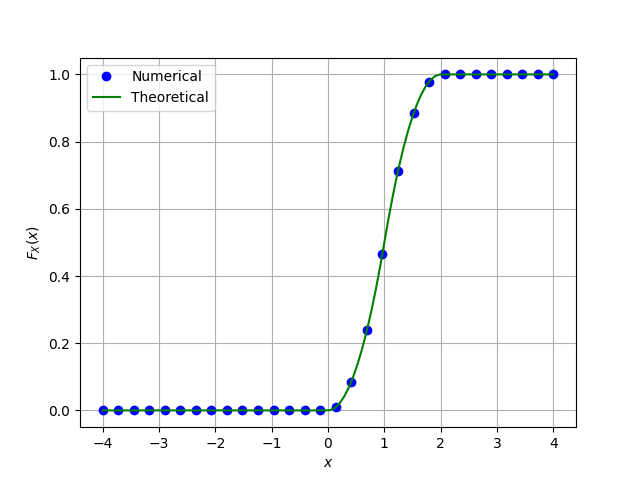
\includegraphics[width=\columnwidth]{../figs/tri_cdf_comp.png}
	\caption{The CDF of $T$}
	\label{fig:TriCDF_2}
	\end{figure}
	
	The plot is shown in figure \eqref{fig:TriCDF_2}

\end{enumerate}

\section{Maximum Likelihood}
\begin{enumerate}[label=\thesection.\arabic*
,ref=\thesection.\theenumi]

\item Generate equiprobable $X \in \cbrak{1,-1}$.
	\\
	\solution
	\\
	We can generate samples for equiprobable random variable $X$ using the following code:
	\begin{lstlisting}
gcc exrand.c -lm
./a.out
	\end{lstlisting}
	The samples generated are stored in \verb|ber.dat|.

\item Generate 
	\begin{equation}
	Y = AX+N,
	\end{equation}
		where $A = 5 \text{dB}, X \in \cbrak{1,-1}$, is Bernoulli and $N \sim \mathcal{N}(0,\,1)$.
	\\
	\solution
	\\
	We can generate samples for random variable $Y$ using the following code:
	\begin{lstlisting}
gcc exrand.c -lm
./a.out
	\end{lstlisting}
	The samples generated are stored in \verb|y.dat|.

\item Plot $Y$.
	\\
	\solution
	\\
	We use the following code to plot all samples of $Y$.
	\begin{lstlisting}
python3 y_plot.py
	\end{lstlisting}
	The plot generated is shown in figure \eqref{fig:YPlot}.

	\begin{figure}
	\centering
	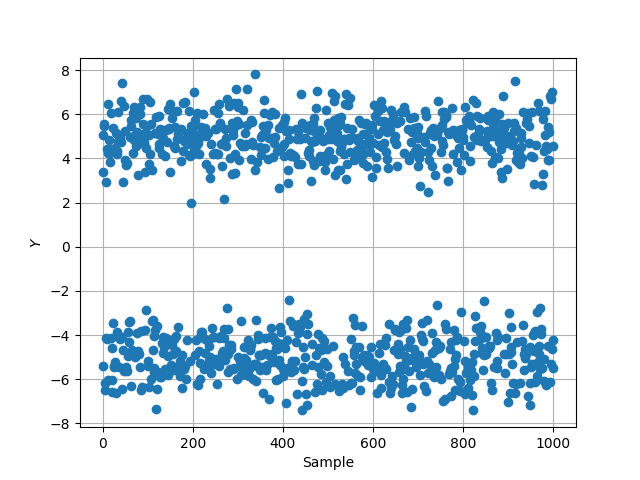
\includegraphics[width=\columnwidth]{../figs/y_plot.png}
	\caption{Random Variable $Y$ at $A = 5.0$}
	\label{fig:YPlot}
	\end{figure}

\item Guess how to estimate $X$ from $Y$.
	\\
	\solution
	\\
	One can roughly estimate $X$ from $Y$ as it is most probable that when $X > 0$, then $Y > 0$. Hence,
	\begin{align}
		X =
		\begin{cases}
			1, & Y > 0 \\
			-1, & Y < 0
		\end{cases}
		\label{eq: Estimate}
	\end{align}

\item
	\label{ml-ch4_sim}
	Find 
	\begin{equation}
		P_{e|0} = \pr{\hat{X} = -1|X=1}
	\end{equation}
	and 
	\begin{equation}
		P_{e|1} = \pr{\hat{X} = 1|X=-1}
	\end{equation}
	\\
	\solution
	\\
	We can use the following code to find $P_{e|0}$ and $P_{e|1}$ as:
	\begin{lstlisting}
gcc exrand.c -lm
./a.out
	\end{lstlisting}

	In the case where $A = 2.5$, we obtain $P_{e|0} = 0.005478$ and $P_{e|1} = 0.005660$.
	
\item Find $P_e$ assuming that $X$ has equiprobable symbols.
	\\
	\solution
	\\
	We can use the following code to find $P_{e}$:
	\begin{lstlisting}
gcc exrand.c -lm
./a.out
	\end{lstlisting}

	In the case where $A = 2.5$, we obtain $P_{e} = 0.005569$.

\item Verify by plotting the theoretical $P_e$ with respect to $A$ from 0 to 10 dB.  
	\\
	\solution
	\\
	\begin{align}
		P_{e|0} &= \pr{\hat{X} = -1|X = 1} \\
		&= \frac{\pr{\hat{X} = -1, X = 1}}{\pr{X = 1}}
	\end{align}

	Using \eqref{eq: Estimate}
	\begin{align}
		P_{e|0} &= \frac{\pr{Y < 0, X = 1}}{\pr{X = 1}} \\
		&= \pr{A + N < 0} \\
		&= \pr{N < -A} \\
		&= 1 - \pr{N \geq -A}\\
		&= 1 - Q(-A)
		\label{eq:PE0}
	\end{align}

	Similarly, we can write
	\begin{align}
		P_{e|1} &= \pr{\hat{X} = 1|X = -1} \\
		&= \frac{\pr{\hat{X} = 1, X = -1}}{\pr{X = -1}} \\
		&= \frac{\pr{Y > 0, X = -1}}{\pr{X = -1}} \\
		&= \pr{-A + N > 0} \\
		&= \pr{N > A} \\
		&= Q(A)
		\label{eq:PE1}
	\end{align}
	
	Hence, we can determine $P_e$ as follows:
	\begin{align}
		P_e &= P_{e|0} \pr{X = 1} + P_{e|1} \pr{X = -1} \\
		&= \frac{1}{2}\left( Q(A) + 1 - Q(-A) \right) \\
		&= \frac{1}{2}\left( 2Q(A) \right) \\
		&= Q(A)
		\label{eq:PE}
	\end{align}

	Note that $\pr{X = 1} = \pr{X = -1} = \frac{1}{2}$ and $Q(A) + Q(-A) = 1$.
	
	We first generate statistically, various values of $P_e$ for different values of $a$. We execute the following code to generate sample:
	\begin{lstlisting}
gcc exrand.c -lm
./a.out
	\end{lstlisting}
	The samples are now generated in \verb|pe_a.dat|.
	
	To observe the theoretical plot and the statistical values of $P_e$ vs $a$, we execute the following code:
	\begin{lstlisting}
python3 pea_graph.py
	\end{lstlisting}

	The plot generated is shown in the figure \eqref{PeaPlot}
	\begin{figure}
	\centering
	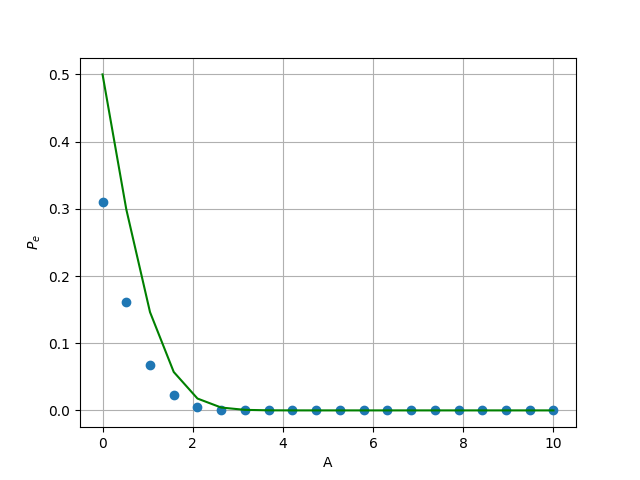
\includegraphics[width=\columnwidth]{../figs/pea_plot.png}
	\caption{$P_e$ vs $a$}
	\label{fig:PeaPlot}
	\end{figure}


	
\item Now, consider a threshold $\delta$ while estimating $X$ from $Y$. Find the value of $\delta$ that minimizes the theoretical $P_e$.
	\\
	\solution
	\\
	Assuming the threshold to be $\delta$, we can estimate $X$ from $Y$:
	\begin{align}
		X =
		\begin{cases}
			1, & Y > \delta \\
			-1, & Y < \delta
		\end{cases}
	\end{align}
	
	In this case
	\begin{align}
		P_{e|0} &= \pr{\hat{X} = -1|X = 1} \\
		&= \frac{\pr{\hat{X} = -1, X = 1}}{\pr{X = 1}} \\
		&= \frac{\pr{Y < \delta, X = 1}}{\pr{X = 1}} \\
		&= \pr{A + N < \delta} \\
		&= \pr{N < \delta - A} \\
		&= 1 - \pr{N \geq \delta - A}\\
		&= 1 - Q(\delta - A)
		\label{eq:PE0Delta}
	\end{align}
	
	Similarly
	\begin{align}
		P_{e|1} &= \pr{\hat{X} = 1|X = -1} \\
		&= \frac{\pr{\hat{X} = 1, X = -1}}{\pr{X = -1}} \\
		&= \frac{\pr{Y > \delta, X = -1}}{\pr{X = -1}} \\
		&= \pr{-A + N > \delta} \\
		&= \pr{N > \delta + A} \\
		&= Q(\delta + A)
		\label{eq:PE1Delta}
	\end{align}
	
	We can write
	\begin{align}
		P_e = P_{e|0} \pr{X = 1} + P_{e|1} \pr{X = -1}
		\label{eq:PEDelta}
	\end{align}
	\begin{align}
		P_e = \frac{1}{2}\left( 1 - Q(\delta - A) + Q(\delta + A) \right)
	\end{align}
	
	To minimise this, we will find the value at $A$ when
	\begin{align}
		\frac{dP_e}{dA} = 0 
	\end{align}
	\begin{align}
		\frac{1}{2} \frac{d}{dA}\left( 1 - Q(\delta - A) + Q(\delta + A) \right) = 0
	\end{align}
	\begin{align}
		\frac{e^{-\frac{\left( \delta - A\right)^2}{2}}}{\sqrt{2\pi}} - \frac{e^{-\frac{\left( \delta + A\right)^2}{2}}}{\sqrt{2\pi}} = 0
	\end{align}
	\begin{align}
		e^{-\frac{\left( \delta - A\right)^2}{2}} = e^{-\frac{\left( \delta + A\right)^2}{2}}
	\end{align}
	\begin{align}
		\frac{\left( \delta - A\right)^2}{2} = \frac{\left( \delta + A\right)^2}{2}
	\end{align}
	\begin{align}
		\left( \delta - A\right)^2 = \left( \delta + A\right)^2
	\end{align}
	\begin{align}
		\delta = 0
		\label{eq:AValue}
	\end{align}
	

\item Repeat the above exercise when 
	\begin{align}
		p_{X}(-1) = p
	\end{align}
	\\
	\solution
	\\
	Using \eqref{eq:PEDelta}, we have:
	\begin{align}
		P_e &= P_{e|0} \pr{X = 1} + P_{e|1} \pr{X = -1} \\
		&= \left(p\right) \left(1 - Q(\delta-A)\right) + \left(1-p\right) \left(Q(\delta+A)\right)
	\end{align}

	We again minimise this, using
	\begin{align}
		\frac{dP_e}{dA} = 0
	\end{align}
	\begin{align}
		\left(p\right) \frac{e^{-\frac{\left( \delta - A\right)^2}{2}}}{\sqrt{2\pi}} - \left(1-p\right) \frac{e^{-\frac{\left( \delta + A\right)^2}{2}}}{\sqrt{2\pi}} = 0
	\end{align}
	\begin{align}
		\frac{p}{1-p} = e^{-2A\delta}
	\end{align}
	\begin{align}
		\delta = \frac{1}{2A} \ln{\frac{1-p}{p}}
	\end{align}
	

\item Repeat the above exercise using the MAP criterion.
	\\
	\solution
	\\
	We can deduce the PDF of X|Y is given by:
	\begin{align}
		p_{X|Y}(x|y) = \frac{p_{Y|X}(y|x) p_X(x)}{p_y(Y)}
		\label{eq:Bayes}
	\end{align}

	Assuming $\pr{X = -1} = p$, we have $p_y(Y)$ using total probability theorem as:
	\begin{align}
		p_y(Y) &= p_{y|x}(Y|1) \pr{X=-1} + p_{y|x}(Y|1) \pr{X=1} \\
		&= \left(p\right) p_y(-A+N) + \left(1-p\right) p_y(A+N) \\
		&= \left(p\right) \frac{e^{-\frac{(y+A)^2}{2}}}{\sqrt{2\pi}} + \left(1-p\right) \frac{e^{-\frac{(y-A)^2}{2}}}{\sqrt{2\pi}}
	\end{align}

	Given a value of $Y = y$, $X = -1$, we have
	\begin{align}
		p_{X|Y}(-1|y) &= \frac{p_{Y|X}(y|-1) p_X(-1)}{p_y(Y)} \\
		&= \frac{\left(p\right) e^{-\frac{(y+A)^2}{2}}}{\left(p\right) e^{-\frac{(y+A)^2}{2}} + \left(1-p\right) e^{-\frac{(y-A)^2}{2}}} \\
		&= \frac{p}{p + \left(1-p\right) e^{2yA}}
		\label{eq:MAP1}
	\end{align}

	Given a value of $Y = y$, $X = 1$, we have
	\begin{align}
		p_{X|Y}(1|y) &= \frac{p_{Y|X}(y|1) p_X(1)}{p_y(Y)} \\
		&= \frac{\left(1-p\right) e^{-\frac{(y-A)^2}{2}}}{\left(p\right) e^{-\frac{(y+A)^2}{2}} + \left(1-p\right) e^{-\frac{(y-A)^2}{2}}} \\
		&= \frac{\left(1-p\right) e^{2yA}}{p + \left(1-p\right) e^{2yA}}
		\label{eq:MAP2}
	\end{align}

	Using \eqref{eq:MAP1} and \eqref{eq:MAP2}, we can conclude:
	\begin{align}
		p_{X|Y}(1|y) > p_{X|Y}(-1|y)
	\end{align}
	when,
	\begin{align}
		\frac{\left(1-p\right) e^{2yA}}{p + \left(1-p\right) e^{2yA}} > \frac{p}{p + \left(1-p\right) e^{2yA}}
	\end{align}
	\begin{align}
		e^{2yA} > \frac{p}{\left(1-p\right)}
	\end{align}
	\begin{align}
		y > \frac{1}{2A} \ln{\frac{p}{\left(1-p\right)}}
		\label{eq:MapCond}
	\end{align}

	Hence, when \eqref{eq:MapCond} holds, we can choose $X = 1$ and $X = -1$ otherwise.

	In the case that $X$ is equiprobable, i.e., $\pr{X = 1} = \pr{X = -1} = \frac{1}{2}$, we consider $p = \frac{1}{2}$.
	Hence, we choose $X = 1$ when
	\begin{align}
		y > \frac{1}{2A} \ln{\frac{0.5}{0.5}} \\
		y > 0
	\end{align}

	Also we choose $X = -1$ when $y \leq 0$.

\end{enumerate}

\section{Gaussian to Other}
\begin{enumerate}[label=\thesection.\arabic*
,ref=\thesection.\theenumi]

\item Let $X_1 \sim \mathcal{N}(0,\,1)$ and $X_2 \sim \mathcal{N}(0,\,1)$. Plot the CDF and PDF of
	
	\begin{equation}
	V = X_1^2 + X_2^2
	\end{equation}
	\\
	\solution
	\\
	We first generate many samples for random variable $V$ as mentioned above, using the following code:
	\begin{lstlisting}
gcc exrand.c -lm
./a.out
	\end{lstlisting}
	The samples generated are stored in \verb|chi.dat|.

	To find the theoretical PDF and CDF for the random variable $V$, we shall assume that $X_1$ and $X_2$ are identical and independent. Now assume that
	\begin{align}
		X_1 = R \cos{\theta} \\
		X_2 = R \sin{\theta}
	\end{align}

	Now, we can see that:
	\begin{align}
		V &= X_1^2 + X_2^2 \\
		&= R^2
		\label{eq:RelationVR}
	\end{align}

	We shall try to transform random variables $X_1$, $X_2$ to polar form, i.e., $r$ and $\theta$, using the Jacobian as follows:
	\begin{align}
		p_{R,\theta}(r, \theta) = |J|p_{X_1, X_2}(x_1, x_2)
		\label{eq:Transform}
	\end{align}
	where
	\begin{align}
		J = \myvec{\frac{\partial x_1}{\partial r}& \frac{\partial x_1}{\partial \theta} \\ \frac{\partial x_2}{\partial r} & \frac{\partial x_2}{\partial \theta}}
	\end{align}

	We find that the Jacobian can be simplified as:
	\begin{align}
		J &= \myvec{ \frac{\partial r \cos{\theta}}{\partial r} & \frac{\partial r \cos{\theta}}{\partial \theta} \\ \frac{\partial r \sin{\theta}}{\partial r} & \frac{\partial r \sin{\theta}}{\partial \theta}} \\
		&= \myvec{\cos{\theta} & -r\sin{\theta} \\ \sin{\theta} & r\cos{\theta}} 
	\end{align}

	Now we can evaluate the determinant as:
	\begin{align}
		|J| &= \left( \cos{\theta} \right)\left( r\cos{\theta} \right) - \left( \sin{\theta} \right)\left( -r\sin{\theta}\right)\\
		&= r
		\label{eq:Jacobian}
	\end{align}

	Since $X_1$ and $X_2$ are independent and identical, we can deduce:
	\begin{align}
		p_{X_1, X_2}(x_1, x_2) = p_{X_1}(x_1)p_{X_2}(x_2)
		\label{eq:Iid}
	\end{align}

	Using \eqref{eq:Jacobian} and \eqref{eq:Iid} in \eqref{eq:Transform}, we can conclude:
	\begin{align}
		p_{r, \theta}(r, \theta) &= r p_{X_1}(x_1) p_{X_2}(x_2) \\
		&= \frac{r}{2\pi}\left( e^{-\frac{x_1^2}{2}} \right)\left( e^{-\frac{x_2^2}{2}}\right) \\
		&= \frac{r}{2\pi}\left( e^{-\frac{x_1^2 + x_2^2}{2}}\right) \\
		&= \frac{r}{2\pi}\left( e^{-\frac{r^2}{2}}\right)
	\end{align}

	Marginal probability $p_R(r)$ can be found as:
	\begin{align}
		p_R(r) &= \int_0^{2\pi} p_{R, \theta}(r, \theta) \, d\theta \\
		&= \int_0^{2\pi} \frac{r}{2\pi} \left( e^{-\frac{r^2}{2}} \right) \\
		&= r e^{-\frac{r^2}{2}}
		\label{eq:R_PDF}
	\end{align}

	Note that $p_R(r)$ is only defined as above only when $r \geq 0$ and is 0 otherwise.

	Hence, we can define distribution $F_R(r)$ as:
	\begin{align}
		F_R(r) &= \pr{R \leq r} \\
		&= \int_{-\infty}^{r} p_R(r) \,dr \\
		&= \int_0^r r e^{-\frac{r^2}{2}} \,dr \\
		&= 1 - e^{-\frac{r^2}{2}}
		\label{eq:R_CDF}
	\end{align}
	when $r \geq 0$ and $0$ when $r < 0$.

	Using \eqref{eq:RelationVR}, we can determine the distribution for random variable $V$:
	\begin{align}
		F_V(x) &= \pr{V \leq x} \\
		&= \pr{R^2 \leq x} \\
		&= \pr{0 \leq R \leq \sqrt{x}} \\
		&= F_R(\sqrt{x})
	\end{align}

	Hence,
	\begin{align}
		F_V(x) =
		\begin{cases}
			1 - e^{-\frac{x}{2}} & x \geq 0 \\
			0 & x < 0
		\end{cases}
		\label{eq:V_CDF}
	\end{align}

	Differentiating this, we obtain the density of random variable $V$:
	\begin{align}
		p_V(x) = 
		\begin{cases}
			\frac{1}{2} e^{-\frac{x}{2}} & x \geq 0 \\
			0 & x < 0
		\end{cases}
		\label{eq:V_PDF}
	\end{align}

	We now plot the statistical and theoretical PDF using the following code:
	\begin{lstlisting}
python3 chi_pdf.py
	\end{lstlisting}
	
	The plot is generated in the figure \eqref{fig:ChiPDF}.
	\begin{figure}
	\centering
	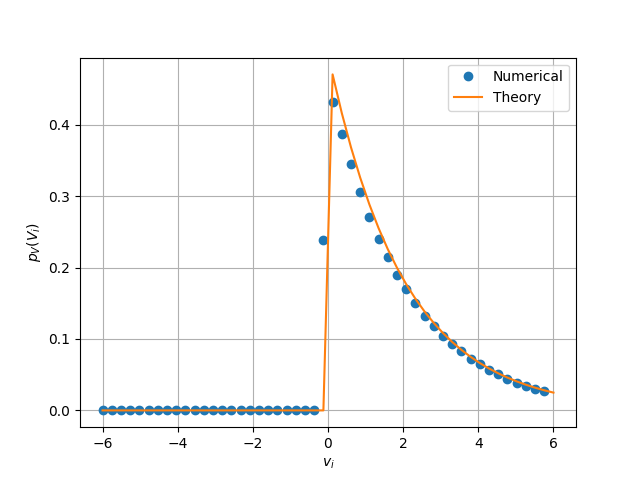
\includegraphics[width=\columnwidth]{../figs/chi_pdf.png}
	\caption{PDF of $V$}
	\label{fig:ChiPDF}
	\end{figure}


	We now plot the statistical and theoretical CDF using the following code;
	\begin{lstlisting}
python3 chi_cdf.py
	\end{lstlisting}

	The plot is generated in the figure \eqref{fig:ChiCDF}
	\begin{figure}
	\centering
	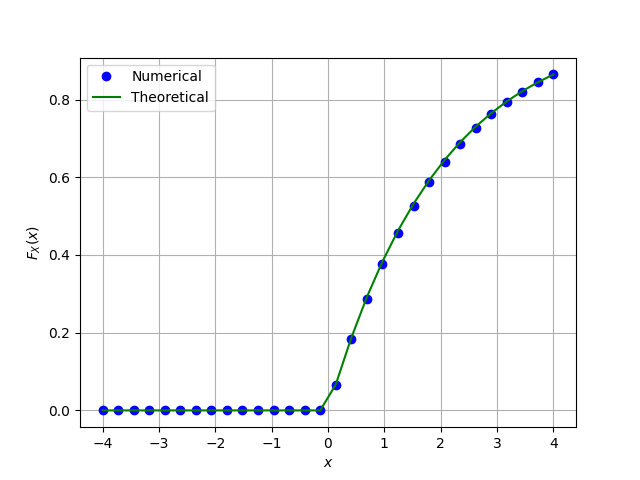
\includegraphics[width=\columnwidth]{../figs/chi_cdf.png}
	\caption{CDF of $V$}
	\label{fig:ChiCDF}
	\end{figure}

\item If
	%
	\begin{equation}
	F_{V}(x) = 
	\begin{cases}
	1 - e^{-\alpha x} & x \geq 0 \\
	0 & x < 0,
	\end{cases}
	\end{equation}
	%
	find $\alpha$.
	%
	\\
	\solution
	\\
	Using \eqref{eq:V_CDF}, we can compare the given equation in the question and obtain
	\begin{align}
		\alpha = \frac{1}{2}
		\label{eq:AlphaVal}
	\end{align}

\item
	\label{ch3_raleigh_sim}
	Plot the CDF and PDF of
	%
	\begin{equation}
	A = \sqrt{V}
	\end{equation}
	%
	\\
	\solution
	\\
	We first generate samples of random variable using the following code:
	\begin{lstlisting}
gcc exrand.c -lm
./a.out
	\end{lstlisting}
	The samples generated are stored in \verb|ray.dat|.
	
	Using these samples we can generate PDF plot using the following code:
	\begin{lstlisting}
python3 ray_pdf.py
	\end{lstlisting}

	The plot generated is shown in figure \eqref{fig:RayPDF}.
	\begin{figure}
	\centering
	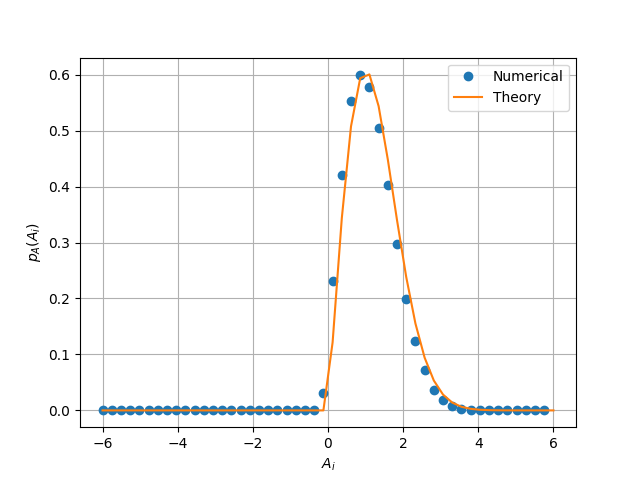
\includegraphics[width=\columnwidth]{../figs/ray_pdf.png}
	\caption{PDF of $A$}
	\label{fig:RayPDF}
	\end{figure}

	Using these samples we can generate PDF plot using the following code:
	\begin{lstlisting}
python3 ray_cdf.py
	\end{lstlisting}

	The plot generated is shown in figure \eqref{fig:RayCDF}.
	\begin{figure}
	\centering
	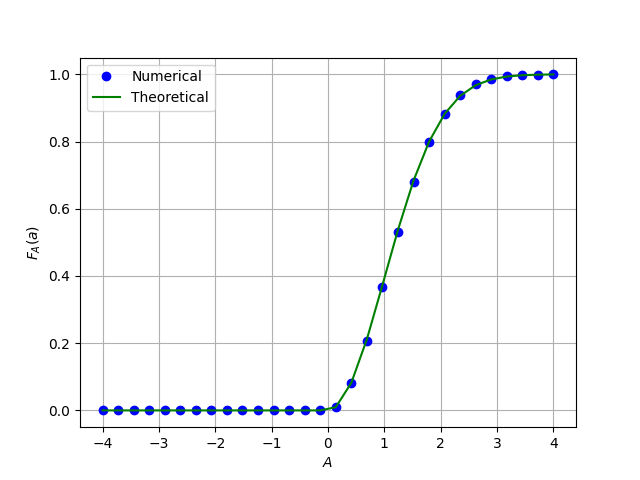
\includegraphics[width=\columnwidth]{../figs/ray_cdf.png}
	\caption{CDF of $A$}
	\label{fig:RayCDF}
	\end{figure}

\end{enumerate}

\section{Conditional Probability}
\begin{enumerate}[label=\thesection.\arabic*
,ref=\thesection.\theenumi]

\item
	\label{ch4_sim}
	Plot 
	\begin{equation}
	P_e = \pr{\hat{X} = -1|X=1}
	\end{equation}
	%
	for 
	\begin{equation}
	Y = AX+N,
	\end{equation}
	where $A$ is Raleigh with $E\sbrak{A^2} = \gamma, N \sim \mathcal{N}(0,\,1), X \in \brak{-1,1}$ for $0 \le \gamma \le 10$ dB.
	%
	
\item
	Assuming that $N$ is a constant, find an expression for $P_e$.  Call this $P_e(N)$
	%
	
\item
	%
	\label{ch4_anal}
	For a function $g$,
	\begin{equation}
	E\sbrak{g(X)} = \int_{-\infty}^{\infty}g(x)p_{X}(x)\, dx
	\end{equation}
	%
	Find $P_e = E\sbrak{P_e(N)}$.
	%
	
\item
	Plot $P_e$ in problems \ref{ch4_sim} and \ref{ch4_anal} on the same graph w.r.t $\gamma$.  Comment.

\end{enumerate}

\section{Two Dimensions}
Let 
\begin{equation}
\mbf{y} = A\mbf{x} + \mbf{n},
\end{equation}
where 
\begin{align}
x &\in \brak{\mbf{s}_0,\mbf{s}_1}, 
\mbf{s}_0 = 
\begin{pmatrix}
1 
\\
0
\end{pmatrix},
\mbf{s}_1 = 
\begin{pmatrix}
0 
\\
1
\end{pmatrix}
\\
\mbf{n} &= 
\begin{pmatrix}
n_1
\\
n_2
\end{pmatrix},
n_1,n_2 \sim \mathcal{N}(0,\,1).
\end{align}
%

\begin{enumerate}[label=\thesection.\arabic*
,ref=\thesection.\theenumi]
%%

\item
	\label{ch5_fsk}
	Plot 
	%
	\begin{equation}
	\mbf{y}|\mbf{s}_0 \text{ and } \mbf{y}|\mbf{s}_1
	\end{equation}
	%
	on the same graph using a scatter plot.
	%
	
\item
	%
	\begin{equation}
	\mbf{y}|\mbf{s}_0 \text{ and } \mbf{y}|\mbf{s}_1
	\end{equation}
	%
	on the same graph using a scatter plot.
	%
	
\item
	For the above problem, find a decision rule for detecting the symbols $\mbf{s}_0 $ and $\mbf{s}_1$.
	%
	
\item
	Plot 
	\begin{equation} 
	P_e = \pr{\hat{\mbf{x}} = \mbf{s}_1|\mbf{x} = \mbf{s}_0}
	\end{equation}
	with respect to the SNR from 0 to 10 dB.
	%
\end{enumerate}
\end{document}
	
